\subsection{Polarization}

A beam of light can be described as a plane electromagnetic wave, like so:
\begin{equation}
    \vec E(z,t)=E_0\cdot\hat e_x\cdot e^{i(\omega t-kz)}
\end{equation}
\begin{equation}
    \vec B(z,t)=B_0\cdot\hat e_y\cdot e^{i(\omega t-kz)}
\end{equation}
The propagation vector $\hat e_z$ together with $\vec E$ and $\vec B$ create 
an orthogonal system. \\ \\ The direction of $\vec E$ defines the polarization, 
which can be distinguished into three types:
\begin{enumerate}
    \centering
    \item linear polarization
    \item elliptical polarization
    \item circular polarization
\end{enumerate}
In the case of elliptical and circular polarisation,
the wave can be  thought of as a superposition of two
orthogonal plane waves with a phase difference $\Delta\varphi=\frac{\pi}{2}$:
\textcolor{red}{What happens for $\Delta\varphi\neq\frac{\pi}{2}$?}
\begin{equation}
    \vec E_\pm=(E_x\hat e_x\mp iE_y\hat e_y)\cdot e^{i(\omega t-kx)}
\end{equation}
If, in addition, both waves carry the same amplitude ($E_x=E_y$),
we speak of circular polarization.

\subsubsection{Snell's law}
If a beam of light reaches the surface between two optical media with
refractive indices $n_1$ and $n_2$, the beam splits into a reflected and a
refracted one. The refraction angle $\alpha_2$ can be determined by
\begin{equation}
    n_1\cdot sin(\alpha_1)=n_2\cdot sin(\alpha_2)
\end{equation}
The angles $\alpha_1$ and $\alpha_2$ are taken between the
incoming/outgoing beam of light and the surface. \\ \\ For reflection,
the condition $\alpha_{in}=\alpha_{out}$ must hold.

\subsubsection{Malus law}
The Malus law states that when a perfect polarizer is placed in a polarized
beam of light, the intensities before and after tranversing the polarizer
are related by
\begin{equation}
    I_f=I_i\cdot cos^2(\theta)
\end{equation}
Here, $\theta$ is the angle between the light's initial polarization
direction and the axis of the polarizer.

\subsubsection{Brewster's angle}
Brewster's angle is a specific angle of incidence at which light with a
particular polarization is perfectly transmitted through a transparent
dielectric surface, without any reflection. \\ \\ When unpolarized light
is incident at this angle, the light that is reflected from the surface is
therefore perfectly polarized. \textcolor{red}{Meaning? Sources?}

\subsubsection{Fresnel equations}
The Fresnel equations describe the reflection and transmission of light
when incident on an interface between different optical media.
\textcolor{red}{equations}

\subsubsection{Reflection and polarization}
Consider again a beam of light traversing from one medium into another.
The beam splits into a reflectd and a refracted part.
From Maxwell's equation the amplitudes and intensities of the two beams
can be derived. The amplitude coefficients corresponding to the reflected and
the transmitted beams are labeled $r$ and $t$. The intensity coefficients
$R$ and $T$ can easily be calculated by taking the square of $r$ and $t$.
If the polarization is perpendicular to the plane of incidence,
the effect is called transversal-electric polarization (German:
S-Polarisation). \\ The coefficients are given by
\begin{equation}
    r_{TE}=-\frac{sin(\alpha_1-\alpha_2)}{sin(\alpha_1+\alpha_2)}
\end{equation}\begin{center}and\end{center}
\begin{equation}
    t_{TE}=\frac{2\cdot sin(\alpha_1)\cdot
    cos(\alpha_2)}{sin(\alpha_1+\alpha_2)}
\end{equation}
If the wave is polarized parallel to the plane of incidence, we speak of
transversal-magnetic polarization (German: P-Polarisation), the coefficients
are given by
\begin{equation}
    r_{TM}=\frac{tan(\alpha_1-\alpha_2)}{tan(\alpha_1+\alpha_2)}
\end{equation}\begin{center}and\end{center}
\begin{equation}
    t_{TM}=\frac{2\cdot sin(\alpha_1)\cdot
    cos(\alpha_2)}{sin(\alpha_1+\alpha_2)\cdot
    cos(\alpha_1-\alpha_2)}
\end{equation}
\begin{figure}[h!]
    \centering
    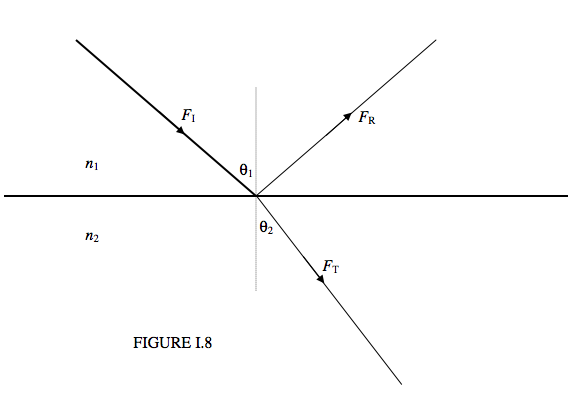
\includegraphics[width=.6\textwidth]{refraction_and_reflection}
    \caption{refraction and reflection}
    \label{refraction_and_reflection}
\end{figure} \\ \textcolor{red}{plot?}

\newpage
\subsubsection{Birefringence}
If the medium is perfectly homogenous and isotropic, the refraction index
is the same in all directions. Here, there is the simple relation
$\vec D=\varepsilon\vec E$ with permittivity $\varepsilon=n^2$.
In general, a medium is likely to be anisotropic. The permittivity
is best described by a tensor $\varepsilon_{ij}$. \\
\textcolor{red}{uniaxial, biaxial media}

\subsubsection{Wave plates}
Wave plates are birefringent crystals used to shift the phase of a
traversing wave by a certain fraction of a whole period. \\ \\
Quarter-wave plates can be used to turn a light beam's polarization
from elliptical to linear and the other way round. For this its
width ideally is $(m+\frac{1}{4})\cdot\lambda, m\in\mathbb{N}$. \\ \\ Half-wave plates
can be used to change the polarization state of linearily polarized
light. The optimal width for this is $(m+\frac{1}{2})\cdot\lambda$.
\begin{figure}[h!]
    \center
    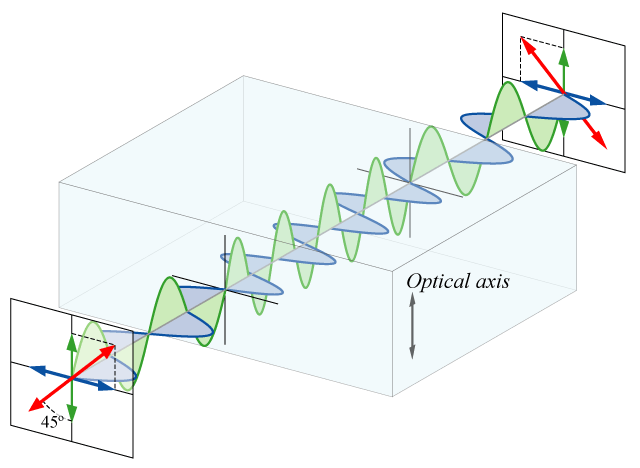
\includegraphics[width=.65\textwidth]{half_wave_plate}
    \caption{effect of a half-wave plate on polarization}
    \label{half_wave_plate}
    %https://upload.wikimedia.org/wikipedia/commons/6/68/Waveplate.png
\end{figure}


\newpage
\subsection{Electro-optical effect}
Some materials experience a change in their optical properties when they are
brought into an external electric field. If the refractive index $n$ is a
function of the applied field $E$, we speak of an electro-optical modulator
(EOM).

\subsubsection{Pockels effect (linear electro-optical effect)}
The refractive index $n=n(E)$ can be expanded around $E=0$
for small field strengths. \\ \\ With
$r=-\frac{2}{n^3}\bigg(\frac{dn}{dE}\bigg)\bigg|_{E=0}$ and
$s=-\frac{1}{n^3}\bigg(\frac{d^2n}{dE^2}\bigg)\bigg|_{E=0}$,
this leads to the relation
\begin{equation}
    n(E)=n_0-\frac{1}{2}rn^3E-\frac{1}{2}sn^3E^2
\end{equation}
The linear electro-optical effect, also called Pockels effect,
occurs for $r\gg s$:
\begin{equation}
    n(E)\approx n_0-\frac{1}{2}rn^3E
\end{equation}
Here, $r$ is called the Pockels coefficient. If, on the other hand, $r\ll s$,
the quadratic dependence of $n$ on $E$ is known as the Kerr effect.
This effect will not be studied in this lab course.

\subsubsection{Pockels effect in a non-isotropic crystal}
Since the electro-optical crystals are in general birefringent, the
Pockels coefficient is not a scalar, but a tensor. For the material
LiNbO$_3$, the entries of this coefficient-tensor are given by
$$\begin{pmatrix}
    r_{11} & r_{12} & r_{13} \\
    r_{21} & r_{22} & r_{23} \\
    r_{31} & r_{32} & r_{33} \\
    r_{41} & r_{42} & r_{43} \\
    r_{51} & r_{52} & r_{53} \\
    r_{61} & r_{62} & r_{63}
\end{pmatrix}=\begin{pmatrix}
    0 & -r_{22} & r_{13} \\
    0 & r_{22} & r_{13} \\
    0 & 0 & r_{33} \\
    0 & r_{51} & 0 \\
    r_{51} & 0 & 0 \\
    -r_{22} & 0 & 0 \\
\end{pmatrix}=\begin{pmatrix}
    0 & -3.4 & 8.6 \\
    0 & 3.4 & 8.6 \\
    0 & 0 & 30.8 \\
    0 & 28 & 0 \\
    28 & 0 & 0 \\
    -3.4 & 0 & 0
\end{pmatrix}\cdot 10^{-12}\ \frac{\textnormal{m}}{\textnormal{V}}$$
If no external field is applied to the crystal, the indicatrix is given by
\begin{equation}
    \frac{1}{n_o^2}x^2+\frac{1}{n_o^2}y^2+\frac{1}{n_e^2}z^2=1
    \label{indicatrix}
\end{equation}
In this lab course, the electric field is applied along the
extraordinary axis of the Pockels cell, the light propagates along one
of the ordinary axes. With $\vec E=E\cdot\hat e_z$ the indicatrix can be
written as
\begin{equation}
    \bigg(\frac{1}{n_0^2}+r_{13}E_z\bigg)x^2+\bigg(\frac{1}{n_0^2}+
    r_{13}E_z\bigg)y^2+\bigg(\frac{1}{n_e^2}+r_{33}E_z\bigg)z^2
\end{equation}
For small applied field strengths this leads to the relations
\begin{equation}
    n_o'(E)\approx n_o-\frac{1}{2}r_{13}n_o^3E_z
    \label{refractive_index_with_pockels_coefficients1}
\end{equation}\begin{equation}
    n_e'(E)\approx n_e-\frac{1}{2}r_{33}n_e^3E_z
    \label{refractive_index_with_pockels_coefficients2}
\end{equation}

\subsubsection{Pockels cell}
An electro-optical crystal between two capacitor plates is called an
electro-optical modulator, abbreviated as EOM. A Pockels cell is an EOM
which exhibits the Pockels effect, meaning that the refractive index is
approximately proportional to the strength of an applied electric field
$\vec E$ (for small values of $|\vec E|$) \\ \\ If light with a wavelength
$\lambda$ travels through a medium with refractive index $n$ for a distance
$L$, the accumulated phase is given by the relation
\begin{equation}
    \Phi=2\pi n\frac{L}{\lambda}
\end{equation}
The phase difference between a beam of light traveling along the ordinary
vs the exraordinary axis is thus:
\begin{equation}
    \Delta\Phi=2\pi(n_e-n_o)\frac{L}{\lambda}
\end{equation}
With a Pockels cell, we can manipulate the magnitude of both $n_o$ and
$n_e$. Plugging equation \ref{refractive_index_with_pockels_coefficients1}
and \ref{refractive_index_with_pockels_coefficients2} into this last
equation, we get the following:
\begin{equation}
    \Delta\Phi(E)=2\pi\frac{L}{\lambda}\bigg(n_e-n_o-\frac{1}{2}
    (r_{33}n_e^3-r_{13}n_e^3-r_{13}n_o^3)E_z\bigg)
\end{equation}
This can be written as
\begin{equation}
    \Delta\Phi(V)=\Phi_0-\pi\frac{V}{V_\pi}
\end{equation}
with $V=Ed$, $\Phi_0=2\pi\frac{L}{\lambda}(n_e-N_o)$ and
$V_\pi=\frac{d}{L}\frac{}{\lambda}{r_{33}n_e^3-r_{13}n_o^3}$
A Pockels cell can be used to modulate the intensity of light. For this, the
cell has to be positioned between two crossed polarizers, each at an
angle of $45^\circ$ relative to the crystal's optical axis.
The transmittance of this setup is
\begin{equation}
    T(V)=sin^2\bigg(\frac{\Phi_0}{2}-\frac{\pi}{2}\frac{V}{V_\pi}\bigg)
\end{equation}

\subsubsection{Faraday effect}
Some media become optically active when an axial magnetic field is applied.
Optically active means that the plane of polarization of linear
polarized light is rotated. The angle of rotation $\alpha_{rot}$ depends
on the length of the medium $L$, the magnetic field strength $|\vec B|$ and
the so-called Verdet constant $v$:
\begin{equation}
    \alpha_{rot}=vL|\vec B|
\end{equation}
The Verdet constant is a function of the wavelength $\lambda$:
\begin{equation}
    v=-\frac{\pi\gamma}{\lambda n}
\end{equation}
Here, $\gamma$ is a material constant of the medium, the so-called
magnetogyration coefficient.

\subsubsection{Optical isolator}
The Faraday effect can be used to build an optical isolator, also called
an optical diode.
\begin{figure}[h!]
    \center
    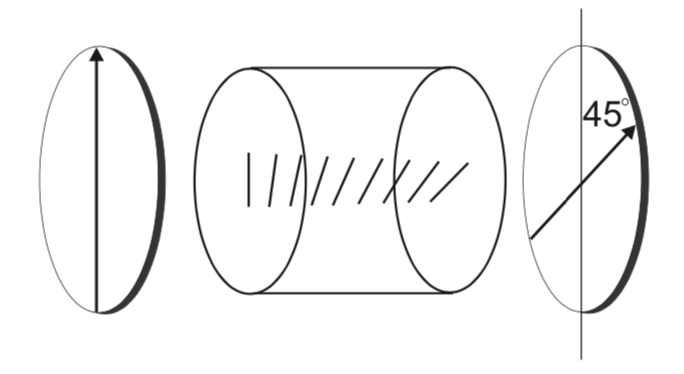
\includegraphics[width=.5\textwidth]{optical_diode}
    \caption{optical diode}
    \label{optical_diode}
\end{figure}


\newpage
\subsection{Acousto-optical effect}
If a sound wave passes through a crystal, its density varies periodically,
which also leads to a periodic variation in the refractive index.
A plane sound wave with wavelength $\lambda_s$ in a crystal with
initial refractive index $n_0$ can be described by
$$n(x,t)=n_0-\Delta n\cdot cos\bigg(\omega t-\frac{2\pi}{\lambda_s}x\bigg)$$
Here, the amplitude $\Delta n=\frac{1}{2}pn^3s_0$ depends on the
photo-elastic constant $p$ and the amplitude of the strain $s_0$.
In this course the main interaction between sound and light will be
the so-called Debye-Sears effect which occurs
%The interaction between laser beam and sound wave occurs either as Bragg
%diffraction for long interaction lengths or as the
for short interaction lengths, i.e. for a thin crystal or thin sound beam.
Parts of the light beam that are travelling through the denser regions
experience a phase shift. Maxima in the far field can be observed, if
these parts of the beam interfere constructively with each other, as can
be seen in the next figure.
\begin{figure}[!h]
\centering
\begin{subfigure}{.5\textwidth}
  \centering
  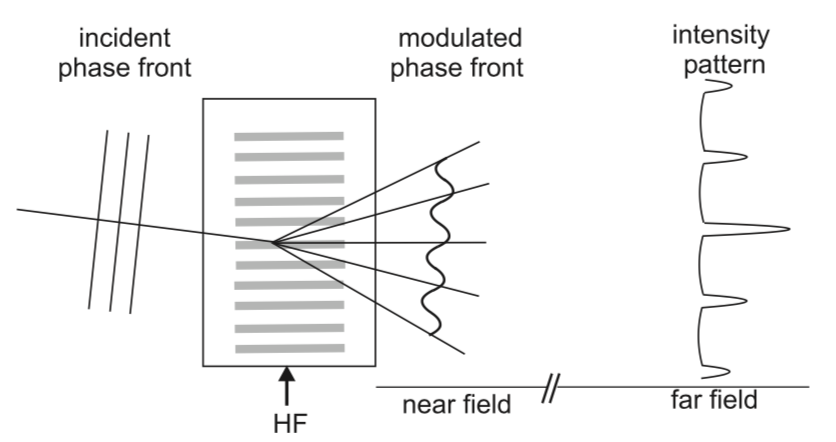
\includegraphics[height=150pt]{acousto_optical_effect_deformation}
  \caption{deformation of a plane wavefront by a sound wave}
  \label{acousto_optical_effect_deformation}
\end{subfigure}%
\begin{subfigure}{.5\textwidth}
  \centering
  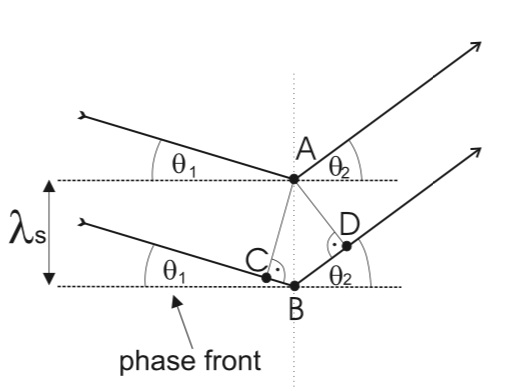
\includegraphics[height=150pt]{acousto_optical_effect_interference}
  \caption{setup 2}
  \label{acousto_optical_effect_interference}
\end{subfigure}
\caption{acousto-optical effect}
\label{acousto_optical_effect}
\end{figure} \\
Because the light is interacting with a moving sound wave, the
diffracted light is Doppler-shifted: $$\textcolor{red}{\omega_{out}=
\omega_{in}+m\Delta\omega=\omega_{in}+m\omega_s}$$
\newpage \noindent
A different approach to explain the effect of an AOM on a light beam is to
describe the system as two scattering quasi-particles, namely a phonon
and a photon. Their momentum vectors are $\hbar\vec k_l$ and $\hbar\vec k_s$,
respectively. Conservation of momentum and energy leads to the relations
$$\vec k_{l,f}=\vec k_{l,i}\pm m\vec k_s$$
\begin{center}and\end{center}
$$\nu_{l,f}=\nu_{l,i}\pm m\nu_s$$
Here, $m$ is the diffraction order, i.e. the number of phonons that
interacted with the photon. Constructive interference occurs when
$$sin\theta_1+sin\theta_2=m\frac{\lambda}{\lambda_s}$$
Here, $\theta_1$ is the angle under which light enters the crystal
and $\theta_2$ the diffraction angle.
\textcolor{red}{efficiency}
